\documentclass{article}
\usepackage[margin=1in]{geometry}
\usepackage[autonum]{tchdr}
\usepackage{graphicx}
\usepackage{listings} %for nice code quoting
\usepackage[sort&compress]{natbib}

%%%%%%%%%%%%%%%%%%%%%%%%%%%%%%%%%%%%%%%%%%
%%Define listings Code format
\definecolor{codegreen}{rgb}{0,0.6,0}
\definecolor{codegray}{rgb}{0.5,0.5,0.5}
\definecolor{codepurple}{rgb}{0.58,0,0.82}
\definecolor{backcolour}{rgb}{0.95,0.95,0.92}

\lstdefinestyle{mystyle}{
	backgroundcolor=\color{backcolour},   
	commentstyle=\color{codegreen},
	%keywordstyle=\color{magenta},
	numberstyle=\tiny\color{codegray},
	stringstyle=\color{magenta},
	basicstyle=\ttfamily\footnotesize,
	breakatwhitespace=false,         
	breaklines=true,                 
	captionpos=b,                    
	keepspaces=true,                 
	numbers=left,                    
	numbersep=5pt,                  
	showspaces=false,                
	showstringspaces=false,
	showtabs=false,                  
	tabsize=2
}

\lstset{style=mystyle}


\title{Preferential Sampling Effect of PM10 in SOCAB Region}
%\author{Xinglong Li \\xinglong.li@stat.ubc.ca}

\begin{document}
\maketitle


\section{Introduction}
In practice, it is common that the selection of locations of sites where the pollutants 
are monitored are affected by the density of the pollutants. It is crucial to take the preferential 
sampling effect into account to accurately model the dispersion of the pollutant and to make 
predictions of pollutants either spatially or into the future.

\cite{Watson2019_pref_samp} proposed a framework that jointly modeling the distribution of an
environmental process and a site-selection process, where the environmental process can be spatial,
temporal, or spatio-temporal. By sharing the random effects between the two process, the joint
model can detect the preferential sampling effects in site selection. 

In this work, we develop an R package for this joint model framework for the purpose of making
spatial predictions. We demonstrate this R package by applying it to the modeling and prediction of
PM10 distributions in California. 
\section{Background}
We consider a spatio-temporal environmental process $Z_{st}$, $s\in \mcS$, $t\in \mcT$.
The space-time point is defined $(s, t) \in \mcS \times \mcT$, where $\mcS$ denoting the spatial 
domain of interest and $\mcT$ the temporal domain. 
Spatial network designer must specify a set of time points $T \subset \mcT$ at which to observe
$Z$ and at each time $t \in T$, a finite subset of sites $S_t \subset \mcS$ at which to do so.

The population of all site locations considered for selection at any time $t \in T$ is defined as 
$\mcP \subset \mcS$, and $\mcP$ is finite and should be specified a priori. 
A Bayesian model is introduced for the joint distribution of the response vector $(Y_{st}, R_{st})$.
$R_{st} \in \{0, 1\}$ is a binary response for the site selection process.
By sharing random effects across the two processes, the stochastic dependence (if any) between 
$Y_{s, t}$ and $R_{s, t}$ and be quantified and subsequently the model can adjust the space-time
predictions according to the preferential sampling effect detected.
Furthermore, in the joint model, the factors affecting the initial site placement can be allowed to
differ from those affecting the retention of existing sites in the network.

\subsection{The joint model}
We let $Y_i(t)$ denote the spatio-temporal observation process at site $i$, that is at locations 
$s_i \in \mcP \subset \mcS$, at time $t \in T$. We let $R_i(t)$ denote the random selection 
indicator for site $s_i \in \mcP$ at time $t$. We let $t_1, \ldots, t_N$ denote the $N$ observation
times, and let $r_{i, j} \in \{0, 1\}$ denote the realization of $R_i(t_j)$, for $i \in \{1, \ldots, M\}$,
$j \in \{1, \ldots, N\}$, where $M = |\mcP|$. The general model framework is
\[
(Y_{i,j} \given R_{i, j} = 1) &\sim f_{Y}(\mu_{i,j}, \theta_Y), \quad f_Y \sim \text{density},\\
g(\mu_{i, j}) = \eta_{i, j} &= \mathbf{x}_{i, j}^T \gamma + \sum_{k=1}^{q_1}u_{i, j, k}\beta_k(s_i, t_j), \\
R_{i, j} &\sim \distBern(p_{i, j}), \\
h(p_{i, j}) &= \nu_{i, j} = \mathbf{v}_{i, j}^T \alpha + \sum_{\ell =1}^{q_2}d_{\ell}\sum_{k=1}^{q_1}
w_{i, j, \ell, k}\beta_k(s_i, \phi_{i, \ell, k}(t_j)) \\
& + \sum_{m=1}^{q_3} w_{i, j, m}^{\star}\beta_m^{\star}(s_i, t_j), \\
\beta_k(s_i, t_j) &\sim \text{(possibly shared) latent effect with parameters}\ \theta_k, \\
& k\in \{1, \ldots, q_1\}, \\
\beta_m^{\star}(s_i, t_j) &\sim \text{site selection only latent effect with parameters}\ \theta_m^\star, \\
& m \in \{1, \ldots, q_3\}, \\
\Theta &= (\theta_Y, \alpha, \gamma, d, \theta_1, \ldots, \theta_{q_1}, \theta_1^{\star}, \ldots, \theta_{q_3}^{\star}) \sim \text{Priors}, \\
\mathbf{x}_{i, j} \in \reals^{p_1}, \mathbf{u}_{i, j} &\in \reals^{q_1}, \mathbf{v}_{i, j} \in \reals^{p_2}, 
\mathbf{W}_{i, j} \in \reals^{q_2\times q_1}, \mathbf{w}_{i, j}^{\star T} \in \reals^{q_3} 
\]

This framework allows a range of different data types of $Y$ to be modeled. In the linear predictor
$\eta_{i, j}$, we include a linear combination of fixed covariates $\bfx_{i, j}$ with 
a linear combination of $q_1$ latent effects $\beta_k(s_i, t_j)$. These $q_1$ random effects
can include any combinations of spatially-correlated processes (such as Gaussian [Markov] random
fields), temporally correlated processes (such as autoregressive terms), spatial temporal processes
and IID random effects. Note that we include the additional fixed covariates $\bfu_{i, j}$ to allow for
spatially-varying coefficient models, as well as both random slopes and/or scaled random effects.

As for the site selection process $R_{i, j}$, the linear predictor $\nu_{i, j}$ may also include 
a linear combination of fixed covariates $\bfv_{i, j}$ with a linear combination of latent effects.
In particular, the latent effects appearing in the observation process $Y_{i, j}$ are allowed to exist
in the linear predictor of the selection process $R_{i, j}$. Note that the matrix $\bfW_{i, j}$ is fixed
beforehand, and allow for $q_2$ linear combinations of the latent effects from the $Y_{i, j}$ 
process to be copied across. The parameter vector $\bfd$ determines the degree to which each shared
latent effect affects the $\bfR$ process and therefore measure the magnitude and direction of stochastic
dependence between the two models term-by-term. We allow $q_3$ latent effects, independent 
from the $Y_{i, j}$ process to exist in the linear predictor.

For added flexibility we allow temporal lags in the stochastic dependence. This allows the 
site-selection process to depend on the realized values of the latent effects at any time arbitrary 
time in the past, present or future. For example, if for a pollution monitoring network, 
site-selection were desired near immediate sources of pollution, then we may view as reasonable, 
a model that allows for a dependence between the latent field at the previous time step 
as a site-selection emulator. In this case, we would select as temporal lag function 
$\phi_{i, \ell, k}(t_j) = t_{j-1}$. 

Also of interest is the possibility of setting $w_{i,j,\ell,m} = 0$ for some values of the subscripts
to allow for the directions of preferentiality to change through time. For example, 
the initial placement of the sites might be made in a positively (or negatively) preferential manner
but over time the network might be redesigned so that sites were later placed to reduce the bias. 
To capture this, it would make sense to have a separate PS parameter $d$ estimated for time $t = 1$
and for times $t > 1$ to capture the changing directions of preferentiality through time. 
This can easily be implemented. Furthermore, we may wish to set $w_{i,j,\ell,m} = 0$ for certain 
values of the subscripts to see if the effects of covariates and/or the effects of preferential sampling 
differs between the initial site placement process and the site retention process.

\subsection{A specific model}
We build one model from the general framework introduced earlier. Let $t_j^{\star}$ denote 
the $j$th time-scaled observations that lie in the interval $[0, 1]$.
The model for the observation process is
\[
(Y_{i, j} \given R_{i, j}=1) &\sim \distNorm(\mu_{i, j}, \sigma_{\epsilon}^2) \\
\mu_{i, j} &= \gamma_0 + \gamma_1 t_j^{\star} + \gamma_2(t_j^{\star})^2 
+ b_{0, i} + b_{1, i}t_j^{\star} 
+ \beta_0(s_i) + \beta_1(s_i)t_j^{\star} + \beta_2(s_i)(t_j^{\star})^2 \label{eq:bs_y}\\
[\beta_k(s_1), \ldots, \beta_k(s_m)]^T &\distiid \distNorm(0, \Sigma(\zeta_k)) \quad 
\text{for}\ k \in \{0, 1, 2\}, \quad \Sigma(\zeta_k) = \text{Matern}(\zeta_k) \\
[b_{0, i}, b_{1, i}]  & \distiid \distNorm(0, \Sigma_b), \quad 
\Sigma_b = \bmat \sigma_{b, 1}^2 & \rho_b  \\ \rho_b & \sigma_{b, 2}^2 \emat, \\ 
\theta &= (\sigma_{\epsilon}^2, \gamma, \zeta_k, \sigma_{b, 1}^2, \rho_b) \sim \text{Priors}.
\]
The model for site-selection process is 
\[
R_{i, j} &\sim \distBern(p_{i, j}) \\
\mathrm{logit}\, p_{i, 1} &= \alpha_{0, 0} + \alpha_1 t_1^{\star} + \alpha_2(t_1^{\star})^2 
+ \beta_1^{\star}(t_1)  \\
& + \alpha_{rep} I_{i, 2} + \beta_0^{\star}(s_i)  \\
& + d_b[b_{0, i} + b_{1, i}(t_1^{\star})] \\
& + d_{\beta}[\beta_0(s_i) + \beta_1(s_i)t_{1}^{\star} + \beta_2(s_i)(t_{1}^{\star})^2], \\
\mathrm{for} j \ne 1 \quad \mathrm{logit}\, p_{i, j} &= \alpha_{0, 1} + \alpha_1 t_j^{\star} + 
\alpha_2 (t_j^{\star})^2 + \beta_1^{\star}(t_j) \\
& + \alpha_{ret}r_{i, (j-1)} + \alpha_{rep} I_{i, j} + \beta_0^{\star}(s_i)  \\
& + d_b[b_{0, i} + b_{1, i}(t_{j-1}^{\star})] \\
& + d_{\beta}[\beta_0(s_i) + \beta_1(s_i)t_{j-1}^{\star} + \beta_2(s_i)(t_{j-1}^{\star})^2], \label{eq:bs_r}\\
I_{i, j} &= \ind\left[ \left( \sum_{\ell\ne i}r_{\ell, j-1}\ind (\|s_i - s_{\ell}\| < c) \right) > 0 \right],\\
[\beta_0^{\star}(s_1), \ldots, \beta_0^{\star}(s_m)]^T &\sim \distNorm(0, \Sigma(\zeta_R)),
\Sigma(\zeta_R) = \mathrm{Matern}(\zeta_R), \\
[\beta_1^{\star}(t_1), \ldots, \beta_1^{\star}(t_T)]^T &\sim \mathrm{AR1}(\rho_a, \sigma_a^2), \\
\theta_R = [\alpha, d_b, d_{\beta}, \rho_a, \sigma_a^2, \zeta_R] & \sim \mathrm{Priors}
\]

The first component is the global effects of time on the log odds of selection. We also add 
first-order autoregressive deviation, $\beta_1^{\star}(t_j)$, from this global quadratic change.
$\alpha_{ret}$ represents the "retention effect" reflecting how the probability a site is selected in a 
given year changes, conditioned on its inclusion in the previous year. Here, we share all parameters
across the two processes and allow only a unique intercept to exist between the processes.
$\alpha_{rep}$ captures the repulsion effect. $I_{i, j}$ denote an indicator variable that determines
whether or not another site in the network placed within a distance $c$ from site $i$ was
was operational at the previous time $t_{j-1}$. We choose the hyperparameter $c$ to be 10 km.

This is a joint model with three processes: an observation process, an initial site-placement process
and a site-retention process. We only allow for a unique intercept to exist across the two processes, 
sharing the remaining parameters. Only the pseudo-sites contribute a zero to the 
Bernoulli likelihood for the site-placement across all years. Only the sites that have been removed 
from the network in year $j$ contribute a zero to the Bernoulli likelihood for the site-retention
process at year $j$. This ensures that no site in the network was ever reinstalled after its removal. 

The latent effects appearing in the observation process $Y_{i, j}$ are allowed to exist
in the linear predictor of the selection process $R_{i, j}$. In particular, the two linear combinations 
of the latent effects, $b_{0, i} + b_{1, i}(t_1^{\star})$ and 
$\beta_0(s_i) + \beta_1(s_i)t_{j-1}^{\star} + \beta_2(s_i)(t_{j-1}^{\star})^2$, from the $Y_{i, j}$ 
process are copied across. The parameters $d_b$ and $d_{\beta}$ determine the degree to which each shared
latent effect affects the $R$ process and therefore measure the magnitude and direction of stochastic
dependence between the two models term-by-term. 

\section{The implementation using inlabru}
To implement the preferential sampling model defined by \cref{eq:bs_y} and \cref{eq:bs_r} 
in INLA, or \textbf{inlabru}, we  are supposed to specify two models. One for the observation 
process in the Gaussian family and one for the site selection process in the Bernoulli family.
Also, we want to share two linear combinations of latent factors between the observation
model and the site selection model:
\[
b_{0, i} + b_{1, i}(t_1^{\star}), \quad \text{and}\quad \beta_0(s_i) + \beta_1(s_i)t_{j-1}^{\star} + \beta_2(s_i)(t_{j-1}^{\star})^2.
\]

While both INLA and \textbf{inlabru} allow copying factors 
between models, each factor (`component' in \textbf{inlabru}) must be copied separately and
therefore introduce one new scale parameter for each copied factor (by setting $fixed = FALSE$). 
In our model, however, 
we only  want two scale parameters $d_b$ and $d_\beta$ for these two linear combinations
of factors:
\[
d_b[b_{0, i} + b_{1, i}(t_1^{\star})]  \quad \text{and }\quad d_{\beta}[\beta_0(s_i) + \beta_1(s_i)t_{j-1}^{\star} + \beta_2(s_i)(t_{j-1}^{\star})^2],
\]
where $d_b$ and $d_{\beta}$ are two scale parameters.
This is not directly achievable using the $copy$ feature in INLA or \textbf{inlabru},
and if we use the $copy$ feature to copy each latent factor separately, 
there will be five (instead of two) new scale parameters introduced at each site and time point. 

\subsection{An alternative approach using auxiliary models}
To copy the linear combinations of factors in implementing the model for black smoke data, \cite{Watson2019_pref_samp}
introduced two auxiliary factors and two auxiliary Gaussian models in addition to the 
original joint model:
\[
0 &= - C_b +  [b_{0, i} + b_{1, i}(t_1^{\star})] \label{eq:bs_aux0} \\
0 &= - C_\beta + [\beta_0(s_i) + \beta_1(s_i)t_{j-1}^{\star} + \beta_2(s_i)(t_{j-1}^{\star})^2] 
\label{eq:bs_aux1}
\]
where $C_b$ and $C_\beta$ are auxiliary latent factors. These individual factors, $b_{0, i}$, $b_{1, i}(t_1^{\star})$, $\beta_0(s_i)$, 
$\beta_1(s_i)t_{j-1}^{\star}$, $\beta_2(s_i)(t_{j-1}^{\star})^2$, are copied separately from the 
observation model \cref{eq:bs_y} to the  two auxiliary models, \cref{eq:bs_aux0} and 
\cref{eq:bs_aux1}, with the argument $fixed = TRUE$. 

By setting the precision parameter of the two factors $C_b$ and $C_\beta$ to be $\approx 0$ and 
setting the precision parameter of the two Gaussian auxiliary models to be $\approx \infty$,
the latent factors $C_b$ and $C_\beta$ duplicate of the two factor combinations:
\[
C_b =  b_{0, i} + b_{1, i}(t_1^{\star})\quad
\text{and} \quad
C_\beta = \beta_0(s_i) + \beta_1(s_i)t_{j-1}^{\star} + \beta_2(s_i)(t_{j-1}^{\star})^2.
\] 
Given the two auxiliary models, the new model for site-selection process copies $C_b$ 
and $C_\beta$ from \cref{eq:bs_aux0} and \cref{eq:bs_aux1} instead with the argument $fixed = FALSE$:
\[
\mathrm{logit}\, p_{i, 1} &= \alpha_{0, 0} + \alpha_1 t_1^{\star} + \alpha_2(t_1^{\star}) 
+ \beta_1^{\star}(t_1)  \\
& + \alpha_{rep} I_{i, 2} + \beta_0^{\star}(s_i)  \\
& + d_b C_b + d_{\beta}C_\beta, \\
\mathrm{for} j \ne 1 \quad \mathrm{logit}\, p_{i, j} &= \alpha_{0, 1} + \alpha_1 t_j^{\star} + 
\alpha_2 (t_j^{\star})^2 + \beta_1^{\star} t_j \\
& + \alpha_{ret}r_{i, (j-1)} + \alpha_{rep} I_{i, 2} + \beta_0^{\star}(s_i)  \\
& + d_b C_b + d_{\beta}C_{\beta}.
\]

With the auxiliary models and factors, it is possible to copy the linear combination of factors 
without introducing too many scale parameters. 
However, this approach requires us to fit four, instead of two models in INLA(or \textbf{inlabru}), 
and in general, more auxiliary models and factors will be required if more linear combinations 
of factors need to be shared between the observation process and the site selection process.

\section{The Preferential Sampling Model}
The population of sites considered for selection should also be selected carefully.
Different choices of the population leads to different conclusions about the PS effect. 
In one case the population is all sites that have been monitored at some times $t \in T$, and
the estimate of the mean value of the PM10 can be interpreted as the network average.
By using this population, the model help us detect the effect of PS on estimates of the density of 
PM10s across all sites ever observed. 
In the other case, we include all vertices of the mesh grid that are inside the border in the 
population and we treat those unobserved vertices as pseudo site locations. These pseudo sites are
placed at a density of approximately 3 km throughout SOCAB region, and in this case, the estimate 
of the mean value of the PM10 in this case can be interpreted as the PM10 density across the SOCAB
region. Since we are uniformly cover the 
SOCAB region, this population help us detect if the observed sites are preferentially selected and 
the effect of PS on estimating the mean of PM10 over the entire SOCAB region.

A Bayesian model is 
introduced for the joint distribution of the response vector $(Y_{st}, R_{st})$, where $R_{st}$ is
a binary response for the site selection process. By sharing random effects across the two processes
the stochastic dependence between the observation and the site selection can be detected and adjust 
the predictions. In particular, the site selection process is allowed to use information from both
spatially varying Gaussian processes and spatially-uncorrelated site-specific effects to determine
the site selection probabilities each year.
We fit the same preferential sampling model for the two populations.


\section{PM10 in California}
The annual concentration of PM10s from 1965 can be download from the website (\url{https://www.epa.gov/outdoor-air-quality-data}) 
of the U.S. Environmental Protection Agency (EPA). We download the annual records of PM10 in California 
between 1985 to 2022. The raw data set include locations, year, and some summery statistics of 
measurements of all sites in California. The complete information of the data set can be found in
the EPA website (\url{https://aqs.epa.gov/aqsweb/airdata/FileFormats.html#_annual_summary_files}).
The raw data set downloaded also include records of other air pollutants, but we keep only the PM10
records.

We keep the annual mean of PM10 measurements to represent the PM10 level at each site.
Sometimes exceptional events happened and can affect the measurements of air pollutants, 
but the local agency has no control over. A wildfire is an example of an exceptional event. 
We use the summary statistics which remove the affects of extreme events.  

The site locations of these sites can be seen from Fig. Note that each measurement site might has 
multiple monitors planted in close but different locations. We combine the measurement of different
monitors of each site by taking the arithmetic average of bothe the locations and PM10 measurements.

The decline trend in concentrations of PM10s from 1965 to can be seen from Fig. The sites are added 
to the network and dropped. It can be seen from the plot that sites remained in the network until 
the end are those with higher measurements.
\subsection{The PM10 Data}
A few data cleaning steps were carried out before fitting the models. Due to the right skewness of 
the PM10 observation distribution, we applied the natural logarithmic transformation to the values
to make the observation more Gaussian in shape. Before the log transformation, we firstly divide
each value by mean of all recorded values to make the response dimensionless.
We scale the Eastings and Northings coordinates and the unit is 100 km. We scaled the years to
lie in the interval $[0, 1]$ to stabilize the temporal polynomials used in later analysis.

\subsection{Data Preprocessing}
In order to make sure the the assumptions on the distributions of data is reasonable, some data
cleaning and preprocessing is required before we fit the PS model. Due to the right skewness of the
PM10 observations, we applied the natural logarithmic transformation to the values to make the 
observations Gaussian distributed. To make the fitted model interpretable, we then subtract the 
logarithmic transformation of the mean value so that the data is dimensionless. 
\begin{figure}[ht]
	\centering
	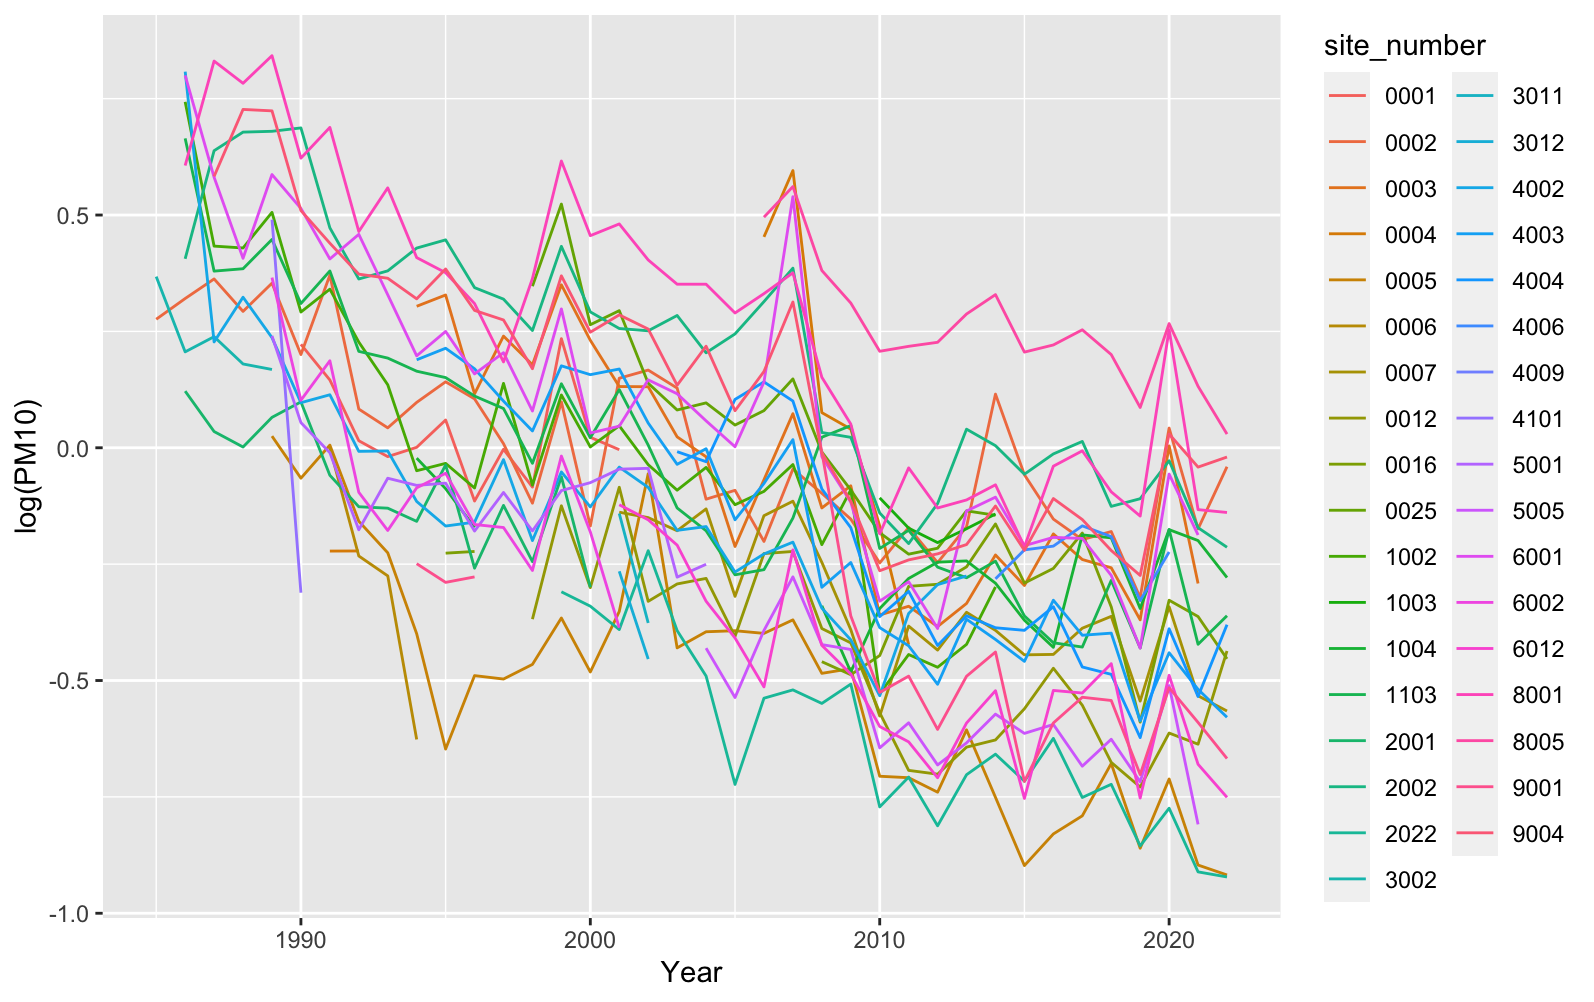
\includegraphics[width = 0.8\textwidth]{socab_plots/logPM10_traces.png}
	\caption{The sites in the SOCAB region.}
	\label{fig:logpm10_traces}
\end{figure}

\begin{figure}[ht]
	\centering
	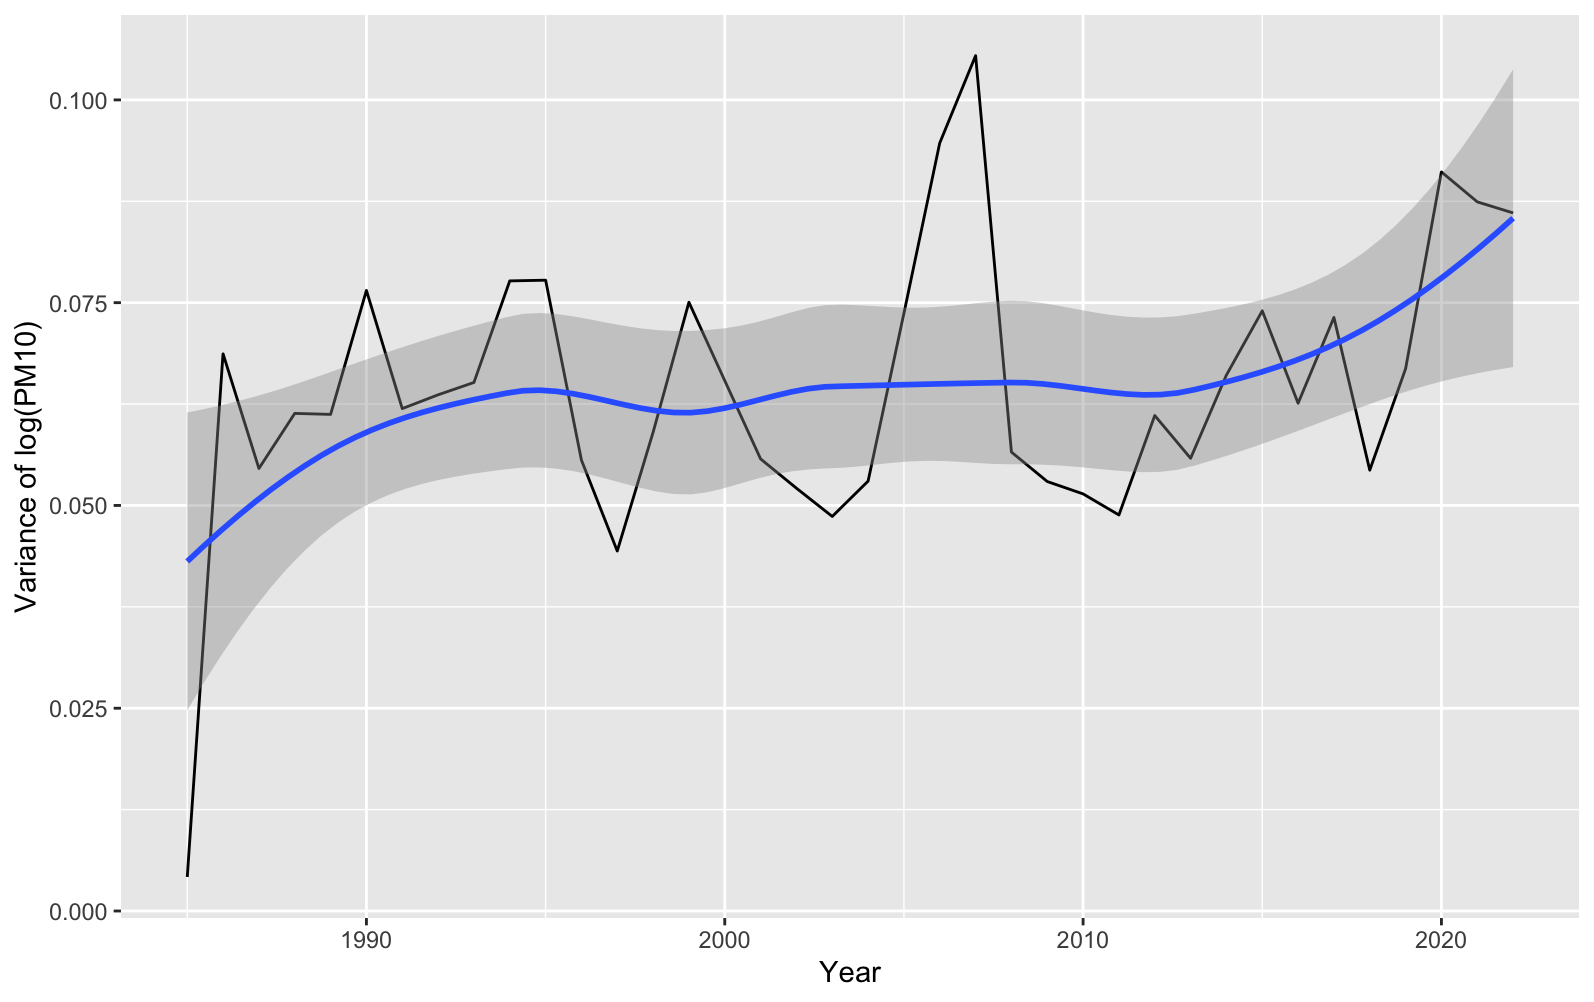
\includegraphics[width = 0.8\textwidth]{socab_plots/logPM10_var.png}
	\caption{The sites in the SOCAB region.}
	\label{fig:logpm10_var}
\end{figure}

\subsection{Map projection and Mesh Grid}
The site locations in the data set are recorded as latitude and longitude under different coordinate
reference systems (CRS). In order to better represent the distance between sites, we project all 
site locations to the UTM (Easting/Northing) coordinates with the measurement unit being kilometer.

The border map of SOCAB region is also projected to the same CRS as the site locations, and we keep
the sites only in the SOCAB region. 

\begin{figure}[ht]
	\centering
	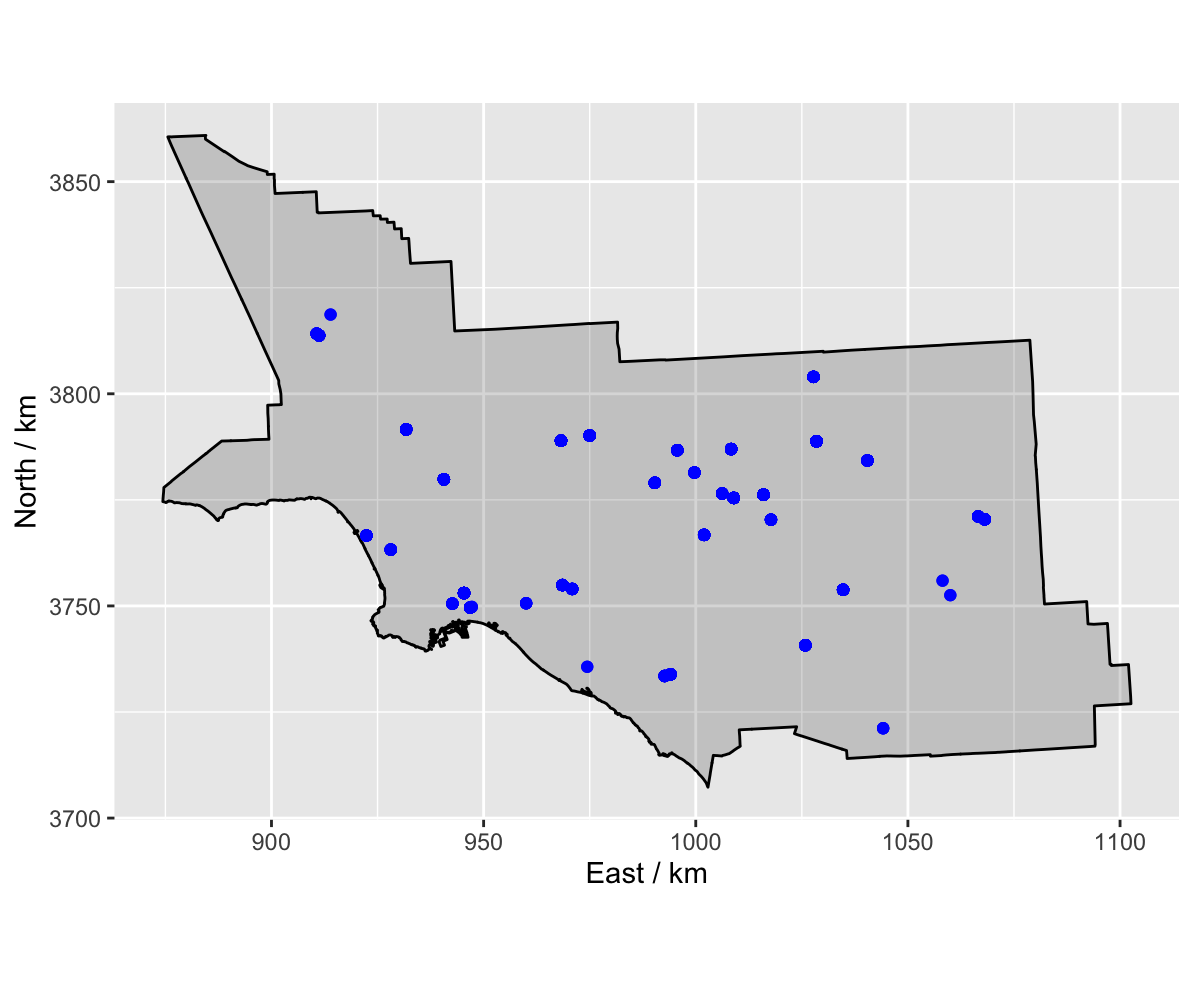
\includegraphics[width = 0.8\textwidth]{socab_plots/SOCAB_sites.png}
	\caption{The sites in the SOCAB region.}
	\label{fig:socab_sites}
\end{figure}

\begin{figure}[ht]
	\centering
	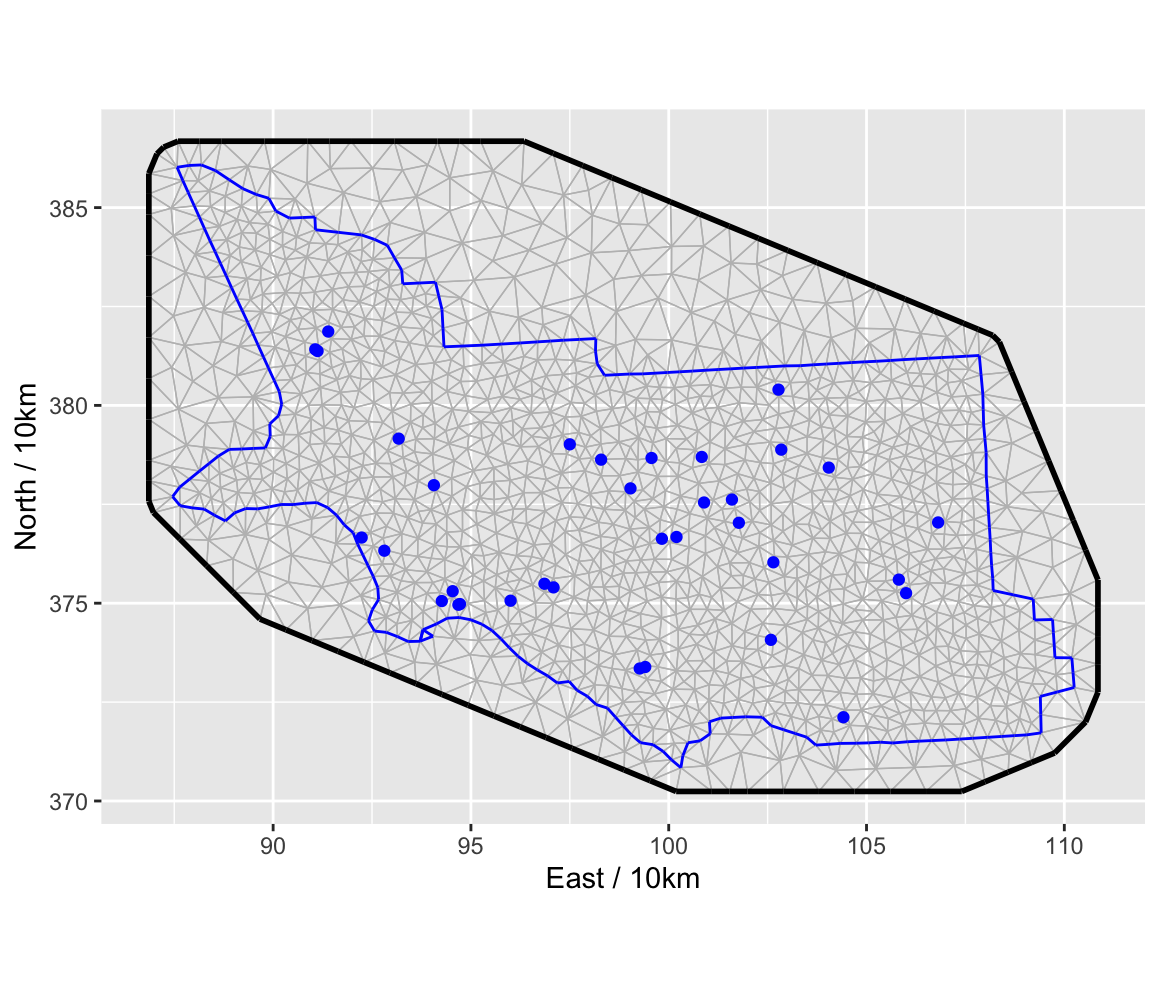
\includegraphics[width = 0.8\textwidth]{socab_plots/SOCAB_meshgrid.png}
	\caption{The meshgrid in the SOCAB region.}
	\label{fig:socab_meshgrid}
\end{figure}

To increase the numerical stability in model fitting, we rescale the Eastings and Northings 
coordinates of sites and the SOCAB border by 10, and each unit distance represent 10 km.

We create the mesh grid using the function $mesh_2d_inla$. 

The same mesh is used in both implementations. 


\section{Model Fitting}
In spatial statistics it is common to formulate mixed-effects regression models in which the linear predictor is made of a trend plus a spatial variation
The trend usually is composed of fixed effects or some smooth terms on covariates, while the spatial variation is usually modeled using correlated random effects.
Spatial random effects often model (residual) small scale variation and this is the reason why these models can be regarded as models with correlated errors.

Lindgren et al. (2011) describe an approximation to continuous spatial models with a Matérn
covariance that is based on the solution to a stochastic partial differential equation (SPDE). 
A Gaussian spatial process with Matérn covariance is a solution to SPDE
This approximation is computed using a sparse representation that can be effectively implemented using the integrated nested Laplace approximation (INLA, Rue et al., 2009)

INLA focuses on models that can be expressed as latent Gaussian Markov random fields (GMRF)

INLA can handle models with more than one likelihood. By using a model with more than one likelihood it is possible to build a joint model with different types of outputs and the hyperparameters in the likelihoods will be fitted separately.

We fit the same model on two populations using R-inlabru package. Inlabru is built upon the R-INLA 
package with simplified syntax. The R-INLA package apply the SPDE approach to add the
This enables the rapid computation of approximate Bayesian posterior distribution of the model 
parameters and random effects. The R-INLA packages approximates the Gaussian Markov random field by
solving an SPDE on a triangulation grid.
The goal of inlabru is to facilitate spatial modeling using integrated nested Laplace approximation via the R-INLA package.

The data set \textbf{PM10s\_SOCAB} has $35 \times 38$ ($\text{number of site} \times \text{number of years}$) 
rows, where each row represent the measurement of one site in a given year. If a site were not
measured in some years, the measurement was noted as missing.  The following variables:
\begin{itemize}
	\item \textbf{annual\_mean}: The logarithmic transformation of annual mean value of PM10s, which acts as the response variable in the regression model.
	\item \textbf{slc}: A dummy variable (0 or 1) indicating whether a site was selected in each year.
	This is the response variable in the site selection model.
	\item \textbf{slc\_lag}: A dummy variable indicating whether a site was selected in last year.
	\item \textbf{site\_number}: The indicator of each site, which is used as the group indicator for random effects
	\item \textbf{locs}: The North/East coordinates (unit 10 km) of sites.
	\item \textbf{year}: The year in which a observation was recorded.
	\item \textbf{time}: The standardized years. 
	\item \textbf{repulsion\_ind}: A dummy variable indicating whether there was other sites in the close neighbor of a site last year.
	\item \textbf{zero}: A vector of zeros that is used as the auxiliary variable in the auxiliary models.
\end{itemize}

We fit the joint model using the R-inlabru package. Our joint model includes four likelihoods, which
includes a Gaussian likelihood for the PM10 concentration process, a binomial likelihood for the
site selection process, and two auxiliary Gaussian likelihoods that are introduced to share linear
combinations of random effects across the PM10 concentration process and the site selection process.

According to the syntax of the R-inlabru package, all components (including the shared ones) of all
likelihoods need to be firstly claimed at once and then used in defining the likelihoods. Each 
effect is defined using a user-assigned name, the variable, and the random distribution. For example


\begin{lstlisting}[language = R]
	components <- ~ 
		# Components for observation model
		intercept_obs(1) +   
		time_1_obs(time) +  
		time_2_obs(time^2) +  
		random_0_obs(site_number, model = "iid2d", n = no_sites*2, constr=TRUE) +  
		random_1_obs(site_number, weights = time, copy = "random_obs0") +  
		spatial_0_obs(locs, model = spde_obj) +  
		spatial_1_obs(locs, weights = time, model = spde_obj) +  
		spatial_2_obs(locs, weights = time^2, model = spde_obj) +    
		# Components for site selection model  
		intercept_slc(1) + 
		time_1_slc(time) +  
		time_2_slc(time^2) +  
		lag_slc(slc_lag) +  
		repuls_slc(repulsion_ind) + 
		ar_slc(year, model='ar1', hyper=list(theta1=list(prior="pcprec",param=c(2, 0.01)))) +  
		spatial_slc(locs, model = spde_obj) +  
		share_aux1(site_number, copy = "comp_aux1", fixed = FALSE) +   
		share_aux2(site_number, copy = "comp_aux2", fixed = FALSE) +    
		# Components for the first auxiliary model  
		random_0_aux1(site_number, copy = "random_obs0", fixed = TRUE) +  
		random_1_aux1(site_number, weights = time, copy = "random_obs11", fixed = TRUE) +  
		comp_aux1(site_number, model = 'iid', 
							hyper = list(prec = list(initial = -20, fixed=TRUE))) +    
		# Components for the second auxiliary model  
		spatial_0_aux2(locs, copy = "spatial_0_obs", fixed = TRUE) +  
		spatial_1_aux2(locs, weights = time, copy = "spatial_1_obs", fixed = TRUE) +  
		spatial_2_aux2(locs, weights = time^2, copy = "spatial_2_obs", fixed = TRUE) +  
		comp_aux2(site_number, model = 'iid', 
							hyper = list(prec = list(initial = -20, fixed=TRUE)))
\end{lstlisting} \label{code:inlabru_components}
\paragraph{The observation likelihood}
We assume that the concentration of PM10s in SOCAB follow a normal distribution. The mean value of 
the concentration is modeled as a combination of a fixed effect and random effects. The fixed 
effect is a quadratic function of time, and the random effects include spatially correlated process,
which is a Gaussian Markov random field, and a site-specific random effect.  

\begin{lstlisting}[language = R]
	like_obs <- like(formula = annual_mean ~ intercept_obs + time_1_obs + time_2_obs +     
																					 random_0_obs + random_1_obs + 
																					 spatial_0_obs + spatial_1_obs + spatial_2_obs,  
									 family = "gaussian",  
									 data = PM10s_SOCAB)
\end{lstlisting} \label{code:inlabru_lik_obs}

The site selection is assumed to follow a Binomial distribution, which is connected to the linear
predictor via a logistic transformation. The fixed effect include a quadratic term and terms 
indicating a site was selected a year before, and a variable indicating the presence of other sites
within certain distance from a site. The random effects including a spatially correlated effect,
and a temporally correlated effect. In order to detect the preferential sampling effect, the random
effects in the observation model are added to the observation process. The shared effects across two
models allow for the stochastic dependence between the two models.

\begin{lstlisting}[language = R]
	like_slc <- like(formula = slc ~ intercept_slc + time_1_slc + time_2_slc +     
																	 lag_slc + repuls_slc + ar_slc + spatial_slc +     
																	 share_aux1 + share_aux2,  
									 family = "binomial",  
									 Ntrials = rep(1, times = length(PM10s_SOCAB$slc)),  
									 data = PM10s_SOCAB)
\end{lstlisting} \label{code:inlabru_lik_slc}

While the R-INLA package and the R-inlabru package allows for components sharing across models, 
sharing of the linear combination of multiple components is not straightforward. To share a linear
combination of components between the two likelihoods, we introduce an auxiliary model with zero 
mean and a vary large variance, and an auxiliary variable to copy the (negative) joint effect of 
the linear combination of multiple effects. 

\begin{lstlisting}[language = R]
	like_aux1 <- like(formula = zero ~ random_0_aux1 + random_1_aux1 + comp_aux1,  
										family = "gaussian",  
										data = PM10s_expand)
\end{lstlisting} \label{code:inlabru_lik_aux1}

\begin{lstlisting}[language = R]
	like_aux2 <- like(formula = zero ~ spatial_0_aux2 + spatial_1_aux2 + spatial_2_aux2 + 
																		 comp_aux2,  
										family = "gaussian",  
										data = PM10s_SOCAB)
\end{lstlisting} \label{code:inlabru_lik_aux2}

\begin{lstlisting}[language = R]
	bru_options_set(bru_max_iter = 20,                
									control.inla = list(strategy = "gaussian", int.strategy = 'eb'),                
									control.family = list(
											list(), 
								    	list(), 
								     	list(hyper = list(prec = list(initial = 20, fixed=TRUE))),                  
								     	list(hyper = list(prec = list(initial = 20, fixed=TRUE)))),                
									bru_verbose = T)
	fit_bru <- bru(components, 
								 like_obs, like_slc, like_aux1, like_aux2)
\end{lstlisting} \label{code:inlabru_fit}

\section{Preferential Sampling Effects}

\clearpage

\bibliographystyle{apalike}
\bibliography{spatial_time}
\end{document}